% This file was created by matlab2tikz.
%
%The latest updates can be retrieved from
%  http://www.mathworks.com/matlabcentral/fileexchange/22022-matlab2tikz-matlab2tikz
%where you can also make suggestions and rate matlab2tikz.
%
\documentclass[]{standalone}
\usepackage{amsmath}
\usepackage{graphicx}
\usepackage[pdf]{pstricks}
\usepackage{pgfplots}
\pgfplotsset{compat=newest}
\usepgfplotslibrary{fillbetween}
%% the following commands are needed for some matlab2tikz features
\usetikzlibrary{plotmarks}
\usetikzlibrary{arrows.meta}
\usepgfplotslibrary{patchplots}
\usetikzlibrary{decorations.text}
\usetikzlibrary{shapes.multipart}


\newcommand{\logLogSlopeTriangle}[5]
{
	% #1. Relative offset in x direction.
	% #2. Width in x direction, so xA-xB.
	% #3. Relative offset in y direction.
	% #4. Slope d(y)/d(log10(x)).
	% #5. Plot options.
	
	\pgfplotsextra
	{
		\pgfkeysgetvalue{/pgfplots/xmin}{\xmin}
		\pgfkeysgetvalue{/pgfplots/xmax}{\xmax}
		\pgfkeysgetvalue{/pgfplots/ymin}{\ymin}
		\pgfkeysgetvalue{/pgfplots/ymax}{\ymax}
		
		% Calculate auxilliary quantities, in relative sense.
		\pgfmathsetmacro{\xArel}{#1}
		\pgfmathsetmacro{\yArel}{#3}
		\pgfmathsetmacro{\xBrel}{#1-#2}
		\pgfmathsetmacro{\yBrel}{\yArel}
		\pgfmathsetmacro{\xCrel}{\xArel}
		%\pgfmathsetmacro{\yCrel}{ln(\yC/exp(\ymin))/ln(exp(\ymax)/exp(\ymin))} % REPLACE THIS EXPRESSION WITH AN EXPRESSION INDEPENDENT OF \yC TO PREVENT THE 'DIMENSION TOO LARGE' ERROR.
		
		\pgfmathsetmacro{\lnxB}{\xmin*(1-(#1-#2))+\xmax*(#1-#2)} % in [xmin,xmax].
		\pgfmathsetmacro{\lnxA}{\xmin*(1-#1)+\xmax*#1} % in [xmin,xmax].
		\pgfmathsetmacro{\lnyA}{\ymin*(1-#3)+\ymax*#3} % in [ymin,ymax].
		\pgfmathsetmacro{\lnyC}{\lnyA+#4*(\lnxA-\lnxB)}
		\pgfmathsetmacro{\yCrel}{\lnyC-\ymin)/(\ymax-\ymin)} % THE IMPROVED EXPRESSION WITHOUT 'DIMENSION TOO LARGE' ERROR.
		
		% Define coordinates for \draw. MIND THE 'rel axis cs' as opposed to the 'axis cs'.
		\coordinate (A) at (rel axis cs:\xArel,\yArel);
		\coordinate (B) at (rel axis cs:\xBrel,\yBrel);
		\coordinate (C) at (rel axis cs:\xCrel,\yCrel);
		
		% Draw slope triangle.
		\draw[#5]   (A)-- node[pos=0.5,anchor=north] {1}
		(B)-- 
		(C)-- node[pos=0.5,anchor=west] {#4}
		cycle;
	}
}

\begin{document}
	
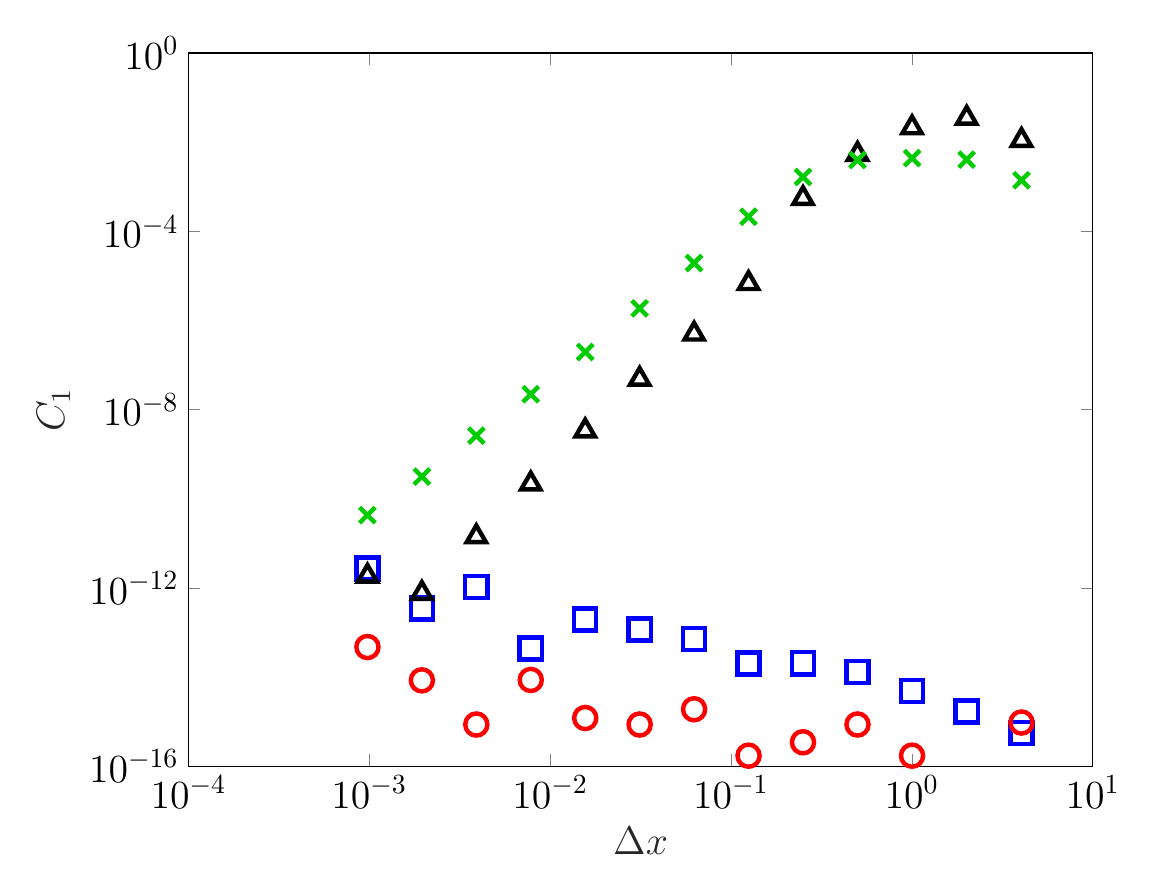
\begin{tikzpicture}
\tikzstyle{every node}=[font=\Large]
\begin{axis}[%
width=4.521in,
height=3.566in,
at={(0.758in,0.481in)},
scale only axis,
every axis plot/.append style={ultra thick},
xmode=log,
xmin=0.0001,
xmax=10,
xtick={0.0001,  0.001,   0.01,    0.1,      1,     10},
xminorticks=false,
xlabel style={font=\color{white!15!black}},
xlabel={\Large $\Delta x$},
ymode=log,
ymin=1e-16,
ymax=1,
ytick={ 1e-16,  1e-12,  1e-08, 0.0001,      1},
yminorticks=false,
ylabel style={font=\color{white!15!black}},
ylabel={\Large $C_1$},
axis background/.style={fill=white}
]

 \logLogSlopeTriangle{0.6}{0.2}{0.3}{3}{black};

\addplot [color=blue, draw=none, mark=square, mark size=4pt, mark options={solid, blue}, forget plot]
  table[row sep=crcr]{%
4.04040404040404	5.59997001419471e-16\\
2.01005025125628	1.68626312842456e-15\\
1.00250626566416	4.93039000236056e-15\\
0.500625782227785	1.31170648191206e-14\\
0.250156347717323	2.04640556548324e-14\\
0.125039074710847	2.01880640876519e-14\\
0.0625097671511174	7.15869808012381e-14\\
0.0312524415969998	1.17202776535745e-13\\
0.0156256103754053	1.96286968428743e-13\\
0.00781265259087092	4.40595128301162e-14\\
0.00390628814734519	1.05757978770092e-12\\
0.00195313453678973	3.45279093058683e-13\\
0.000976564884191612	2.73611397070572e-12\\
};
\addplot [color=red, draw=none, mark=o, mark size=4pt, mark options={solid, red}, forget plot]
  table[row sep=crcr]{%
4.04040404040404	9.55567593565475e-16\\
2.01005025125628	0\\
1.00250626566416	1.7269095955102e-16\\
0.500625782227785	8.63313252681634e-16\\
0.250156347717323	3.45325301041395e-16\\
0.125039074710847	1.72662650520698e-16\\
0.0625097671511174	1.89928915572767e-15\\
0.0312524415969998	8.63313252603487e-16\\
0.0156256103754053	1.20863855364489e-15\\
0.00781265259087092	8.63313252603496e-15\\
0.00390628814734519	8.63313252603497e-16\\
0.00195313453678973	8.46046987551437e-15\\
0.000976564884191612	4.73095662426736e-14\\
};
\addplot [color=black, draw=none, mark=triangle, mark size=4pt, mark options={solid, black}, forget plot]
  table[row sep=crcr]{%
4.04040404040404	0.0110209325923989\\
2.01005025125628	0.0346913505175811\\
1.00250626566416	0.0211526678655773\\
0.500625782227785	0.00536098541759149\\
0.250156347717323	0.000547721210121052\\
0.125039074710847	6.7842541844407e-06\\
0.0625097671511174	4.98395192794452e-07\\
0.0312524415969998	4.83428048001805e-08\\
0.0156256103754053	3.35530354823315e-09\\
0.00781265259087092	2.16657932193184e-10\\
0.00390628814734519	1.41992636392536e-11\\
0.00195313453678973	7.59543069826154e-13\\
0.000976564884191612	1.84300117423292e-12\\
};
\addplot [color=green!80!black, draw=none, mark=x, mark size=4pt, mark options={solid, green!80!black}, forget plot]
  table[row sep=crcr]{%
4.04040404040404	0.00140499199671105\\
2.01005025125628	0.00405828379198588\\
1.00250626566416	0.00439334485366716\\
0.500625782227785	0.00398769442286889\\
0.250156347717323	0.00165335248268688\\
0.125039074710847	0.000213116754236917\\
0.0625097671511174	1.94733957415532e-05\\
0.0312524415969998	1.86605467379564e-06\\
0.0156256103754053	1.95846174482759e-07\\
0.00781265259087092	2.21165256489069e-08\\
0.00390628814734519	2.61638977810564e-09\\
0.00195313453678973	3.15849947329427e-10\\
0.000976564884191612	4.30412056752375e-11\\
};
\end{axis}
\end{tikzpicture}%
\end{document}